\chapter{Introduction}
    Our idea for the 3D Computer Vision mini project was to create high quality 3D reconstructions from regular smartphone videos, without the need for an expensive RGB-D camera like the Microsoft Kinect.
    To make this feasible, we try to combine fine-tuned depth map estimates from Convolutional Neural Networks (CNNs) with state of the art RGBD-SLAM methods.\\
    For the estimation of the depth maps we rely on the approach of Luo et al. \cite{luo2020consistent} (\citetitle{luo2020consistent}) to fine-tune the monocular depth estimation model from Google, which was initially trained on the Mannequin Challenge dataset \cite{mannequin}.
    Their method addresses the usual problems of monocular depth estimation and promises to produce plausible, geometrically and temporally consistent depth maps for any input video, which is a key element for high-quality reconstructions.
    This method provides us with our depth estimates, as well as relatively accurate camera extrinsics and intrinsics. The latter are obtained from bundle adjustment of sparse SIFT points using COLMAP \cite{colmap}.\\
    These are the initial values for our reconstruction approach that is strongly based on the Bundle Fusion paper \cite{dai2017bundlefusion} by Dai et al..
    They are proposing a two-step (sparse then dense) pose optimization with a strong focus on real-time applicability.
    As the fine-tuning of the depth estimates cannot be done in real-time, we are only interested in their optimization strategies.
    To be more specific, we only apply their fine-scaled dense optimization strategy for pixel-level alignment of the frames. Their hierarchical sparse optimization has the primary focus of real-time applicability, and does not yield higher accuracy than our exhaustively matched points acquired from COLMAP.
    This dense optimization is based on an energy minimization approach that tries to minimize the average photo- and geometric pixel error. Assuming decent depth estimates, the error should come from the slightly incorrect camera rotations and translations.
    Finally we use Open3D \cite{open3d} to integrate the RGB and depth frames into a scalable truncated signed distance function (TSDF) voxel volume with the optimized camera trajectory. Open3D gives us some handy features and allows us to easily extract textured meshes from these volumes for visualization.

    \begin{figure}[!hb]
        \centering
        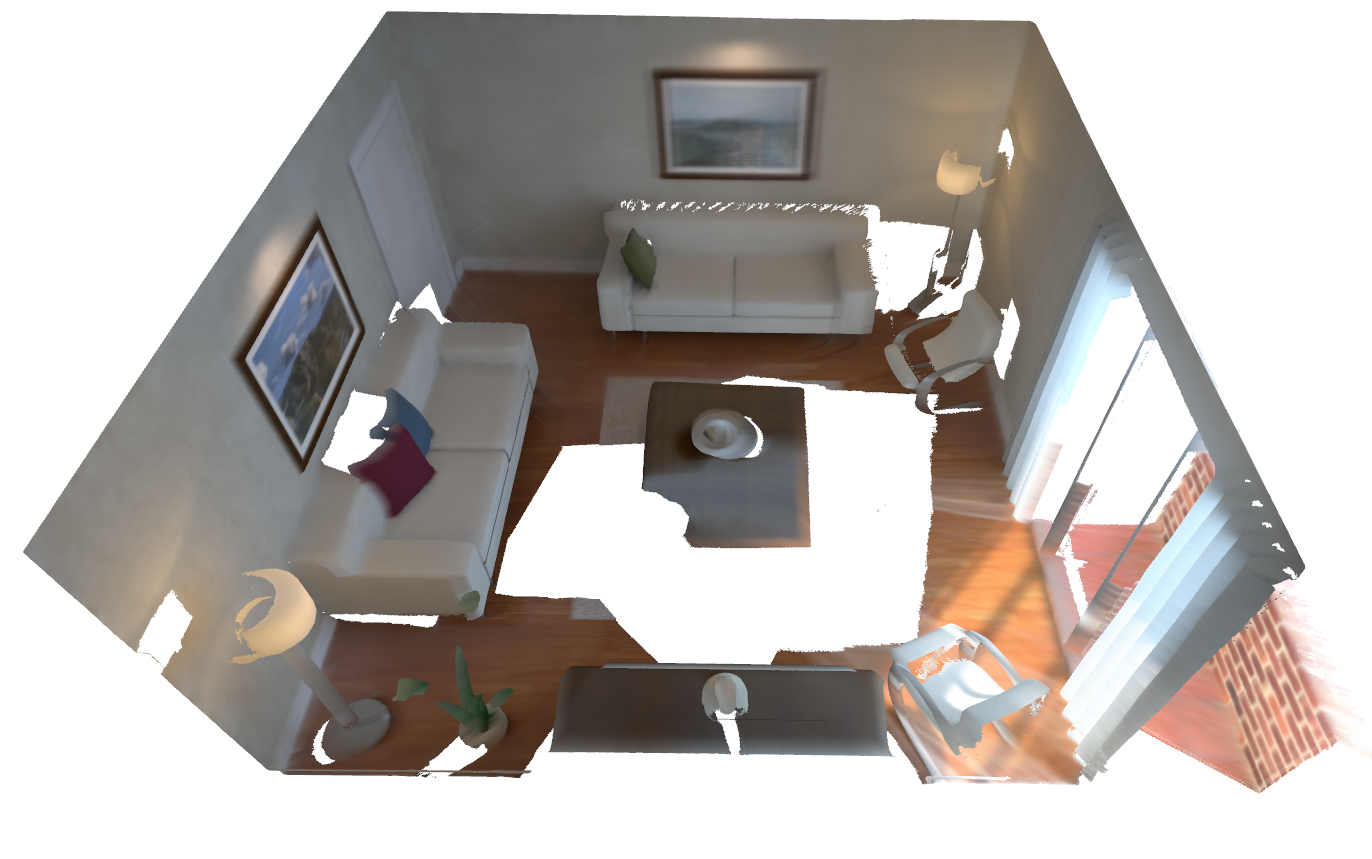
\includegraphics[width=0.6\textwidth]{images/gt_reconstruction.png}
    \end{figure}